% packages
\PassOptionsToPackage{dvipsnames}{xcolor}  % needed to get colors working in certain environments
\documentclass[titlepage,11pt,a4paper,ngerman]{article}
\usepackage[utf8]{inputenc}
\usepackage[T1]{fontenc}
\usepackage[german]{babel}
\usepackage{graphicx}
\usepackage{wrapfig}  % used for wrapping a figure alternative to using minipages
\usepackage{amsmath}
\usepackage{amsfonts}
\usepackage{amssymb}
\usepackage[hidelinks]{hyperref}  % removes coloring for links
\usepackage{cleveref}
\usepackage{tikz}
\usepackage{tikz-cd}
\usepackage{nicefrac}  % adds \nicefrac alternative to regular \frac
\usepackage{mathtools}
\usepackage{enumerate}
\usepackage{cancel}  % adds \cancel which adds strikethrough
\usepackage{tocloft}
\usepackage{tcolorbox}
\usepackage{bm}  % adds \bm to make symbols bold, replaces outdated \boldsymbol
\usepackage[shortlabels]{enumitem}
\usepackage{placeins}
\usepackage{booktabs}
\usepackage{wasysym}

\usepackage[margin=1in]{geometry}  % changes the margins on all pages
\usepackage{url}

%SI-unix
%\usepackage{array}
\usepackage[per=slash,
            decimalsymbol=comma,
			loctolang={DE:ngerman,UK:english},
			]{siunitx}	
\sisetup{locale = DE}

\usetikzlibrary{calc}
\usetikzlibrary{decorations.pathmorphing,patterns}
\usetikzlibrary{arrows}
\usetikzlibrary{decorations.pathreplacing}
%\usetikzlibrary{snakes}

% Andrez:
%\usepackage{epigraph}  % adds \epigraph used to add fancy quotes to the beginning of chapters
%\usepackage{fancyhdr}
%\setlength{\parskip}{1em}
%\setlength{\headheight}{35pt}
%\setlength\epigraphwidth{.8\textwidth}
% alt math font
%\usepackage{eulervm}  % switches to alternate math font, usually requires extra download


%Environments und Newcommands:


% general commands

% zu zeigen symbol
\newcommand{\zz}{\fontfamily{cmss} \selectfont{Z\kern-.61em\raise-0.7ex\hbox{Z}:}}
% build over
\newcommand{\bov}[2]{\buildrel{#2} \over{#1}}
% better looking := (defined as)
\newcommand*{\defeq}{\mathrel{\vcenter{\baselineskip0.5ex \lineskiplimit0pt \hbox{\scriptsize.}\hbox{\scriptsize.}}}=}
\newcommand*{\eqdef}{=\mathrel{\vcenter{\baselineskip0.5ex \lineskiplimit0pt \hbox{\scriptsize.}\hbox{\scriptsize.}}}}

% integral differential d
\newcommand{\dif}{\mathop{}\!\mathrm{d}}
\newcommand{\difi}[1]{\mathrm{d}#1\mathop{}\!}

\newcommand{\prt}[2]{\frac{\partial #1}{\partial #2}}  % used for partial derivatives, tip: input #1 can be left blank
\newcommand{\prd}[2]{\frac{\tx{d} #1}{\tx{d} #2}}  % used for absolute (standart) derivatives, tip: input #1 can be left blank

\newcommand{\dd}{\tx{d}}


%Mathe:
\newcommand{\verteq}{\rotatebox{90}{$\,=$}}  % used for commands below
\newcommand{\equalto}[2]{\underset{\scriptstyle\overset{\mkern4mu\verteq}{#2}}{#1}}  % adds equal to underneath
\newcommand{\equaltoup}[2]{\overset{\scriptstyle\underset{\mkern4mu\verteq}{#2}}{#1}}  % adds equal to above
\newcommand{\custo}[3]{\underset{\scriptstyle\overset{\mkern4mu\rotatebox{-90}{$\,#1$}}{#3}}{#2}}  % same as above but replaces equal sign with input #1
\newcommand{\custoup}[3]{\overset{\scriptstyle\underset{\mkern4mu\rotatebox{-90}{$\hspace{-3pt} #1$}}{#3}}{#2}}
\newcommand{\casess}[4]{\left\{ \begin{array}{ll} {#1} & {#2} \\ {#3} & {#4} \end{array} \right.}  % used to indicate to the reader that something is missing here


%Text:
\newcommand{\tx}[1]{\textrm{#1}}
\newcommand{\const}{\tx{const.}}

\newcommand{\ul}[1]{\underline{#1}}
\newcommand{\ol}[1]{\overline{#1}}
\newcommand{\ub}[1]{\underbrace{#1}}
\newcommand{\ob}[1]{\overbrace{#1}}

\newcommand{\hfw}{\color{RubineRed}\tx{ $\star$hier fehlt was$\star$ } \color{black}}  % used to indicate to the reader that something is missing here 


%Spezielles:


%Theo:
\newcommand{\lag}{\mathcal{L}}  % used for Lagrange function
\newcommand{\ham}{\mathcal{H}}  % used for Hamiltonian function
\newcommand{\gre}{\mathcal{G}}  % used for Green's function
\newcommand{\eofr}{\vec{E}(\vec{r})}
\newcommand{\pofr}{\Phi(\vec{r})}
\newcommand{\grr}{\mathcal G(\vec{r},\vec{r}')}
\newcommand{\vphi}{\varphi}
\newcommand{\vabla}{\vec{\nabla}}


%LA:
\newenvironment{bew}[1]{\subsection{Bew: #1}}{\hfill$\square$}
\newcommand{\Bew}[2]{\begin{bew}{#1}#2\end{bew}}
\newcommand{\enph}{F: V \to V \textrm{ Endomorphismus}}

\newcommand{\im}{\tx{im}}
\newcommand{\spa}{\tx{span}}
\newcommand{\adj}{\tx{adj}}
\newcommand{\grad}{\tx{grad}}
\newcommand{\ord}{\tx{ord}}

\newcommand{\basis}[3]{\{#1_{#2}, \dots, #1_{#3}\}}
\newcommand{\ska}[2]{\langle #1 , #2 \rangle}  % scalar product of input 1, and 2 can also be used for braket notation
\newcommand{\dmat}[3]{\begin{pmatrix} #1_{#2}&&\\ &\ddots& \\ && #1_{#3} \end{pmatrix}}


%Ex:
\newcommand{\kq}{\frac{1}{4\pi\epsilon_0}}  % writes out the whole constant k from electrostatic
\newcommand{\kqq}{\frac{\mu_0}{4\pi}}  % writes out the constant from magnetostatic
\newcommand{\uind}{U_{\tx{ind}}}
\newcommand{\folie}[1]{\color{gray}[Folie: #1]\color{black}}  % used to tell the reader that there was multimedia content during a lecture
\newcommand{\versuch}[1]{\color{red!50!black} \textbf{Versuch:} \color{black} \textbf{#1}\\ }  % used to tell the reader that there was a live experiment

\newcommand{\mau}{$\buildrel \mathcal{O} \over{\textbf{.}}$}  % the extreme Waldmann exclamation mark recreated in latex by Markus


% Lab commands:
\newcommand\mean{\begin{equation}
\frac{\sum_{i=1}^n x_i}{n}\label{mean}
\end{equation}}  % shortcut for the standard Mean function

\newcommand\meanstd{\begin{equation}
s_x=\sqrt{\frac{1}{n-1}\sum_{i=1}^n(x_i-\overline{x})^2}\label{meanstd}
\end{equation}}  % shortcut for the standard derivative mean function

\newcommand\prodquo{\begin{equation}\left\vert\frac{\Delta z}{z}\right\vert=\sqrt{\left(a\frac{\Delta x}{x}\right)^2+\left(b\frac{\Delta y}{y}\right)^2+\ldots}\textrm{ f\"ur }z=x^a\ y^b\ldots\end{equation}}

\newcommand\tfuncd{\begin{equation}
t=\frac{\vert x_n-y_n\vert}{\sqrt{x_s^2+y_s^2}}
\end{equation}}

\newcommand\tfunc{\begin{equation}
t=\frac{\vert x-y_0\vert}{u_x}
\end{equation}}


% ANDREZ
%\newcommand{\summ}[2]{\sum_{#1}^{#2}}
%\newcommand{\intt}[2]{\int_{#1}^{#2}}
\newcommand{\lcom}[1]{\color{MidnightBlue}#1\color{black}}  % used to indicate to the reader that this content was transcribed from the lecture
\newcommand{\bei}{\emph{Beispiel:}}
\newcommand{\bem}{\emph{Bemerkung:}}


% Boxen:

\tcbuselibrary{theorems}

% mahlt eine box nur um den text mit titel
\newtcbox{\fribox}[1]{nobeforeafter,colback=white,colframe=red!75!black,fonttitle=\bfseries,title=#1,sharp corners,tcbox raise base}

% mahlt eine große box um alles mit titel
\newcommand{\frbox}[2]{\begin{tcolorbox}[colback=white,colframe=red!75!black,fonttitle=\bfseries,title=#1]#2\end{tcolorbox}}

% mahlt eine box nur um den text
\newtcbox{\ribox}{nobeforeafter,colback=white,colframe=red!75!black,sharp corners,tcbox raise base}

% mahlt eine große box um alles was drinnen ist
\newcommand{\rbox}[1]{\begin{tcolorbox}[colback=white,colframe=red!75!black]#1\end{tcolorbox}}

% mahlt eine box um mathe innerhalb mathmode
\newcommand{\rmbox}[1]{\tcboxmath[colback=white,colframe=red!75!black]{#1}}

% super box (looks like regular boxed but wraps around anything)
\newenvironment{supbox}{\begin{tcolorbox}[colback=white,colframe=black,sharp corners,boxrule=.5pt]}{\end{tcolorbox}}

% the Big Black Box, can be used to separate examples or review material from the main text (used for Wiederholung)
\newcommand{\bbb}[2]{\begin{tcolorbox}[colback=white,colframe=black,fonttitle=\bfseries,title=#1,sharp corners,tcbox raise base]#2\end{tcolorbox}}

% array type box with title
\newenvironment{zebox}[1]{\begin{array}{|c|}
		\multicolumn{1}{l}{\tx{#1}} \\
		\hline
		\displaystyle
	}{\\ \hline
\end{array}}

% arrow list
\newlist{arrowlist}{itemize}{1}
\setlist[arrowlist]{label=$\Rightarrow$}


% optional:

\renewcommand{\vec}[1]{\bm{#1}}

% changed because of preferred looks
\renewcommand{\epsilon}{\varepsilon}
\renewcommand{\paragraph}[1]{\subsubsection{#1}}  % changed oddly behaving paragraphs to simple subsubsections which are not numbered nor in the toc

% nur in Theo benutzt !!!
% \renewcommand{\Phi}{\varPhi}

% evtl:
% \renewcommand{\boxed}{\rmbox}


% Tikz definitions:

\def\centerarc[#1](#2)(#3:#4:#5)% Syntax: [draw options] (center) (initial angle:final angle:radius)
{ \draw[#1] ($(#2)+({#5*cos(#3)},{#5*sin(#3)})$) arc (#3:#4:#5); }

\def\checkmark{\tikz\fill[scale=0.4](0,.35) -- (.25,0) -- (1,.7) -- (.25,.15) -- cycle;}  % checkmark used for proofs

\tikzset{
	annotated cuboid/.pic={
		\tikzset{%
			every edge quotes/.append style={midway, auto},
			/cuboid/.cd,
			#1
		}
		\draw [every edge/.append style={pic actions, densely dashed, opacity=.5}, pic actions]
		(0,0,0) coordinate (o) -- ++(-\cubescale*\cubex,0,0) coordinate (a) -- ++(0,-\cubescale*\cubey,0) coordinate (b) edge coordinate [pos=1] (g) ++(0,0,-\cubescale*\cubez)  -- ++(\cubescale*\cubex,0,0) coordinate (c) -- cycle
		(o) -- ++(0,0,-\cubescale*\cubez) coordinate (d) -- ++(0,-\cubescale*\cubey,0) coordinate (e) edge (g) -- (c) -- cycle
		(o) -- (a) -- ++(0,0,-\cubescale*\cubez) coordinate (f) edge (g) -- (d) -- cycle;
		\path [every edge/.append style={pic actions, |-|}]
		%(b) +(0,-5pt) coordinate (b1) edge ["\cubex \cubeunits"'] (b1 -| c)
		%(b) +(-5pt,0) coordinate (b2) edge ["\cubey \cubeunits"] (b2 |- a)
		%(c) +(3.5pt,-3.5pt) coordinate (c2) edge ["\cubez \cubeunits"'] ([xshift=3.5pt,yshift=-3.5pt]e)
		;
	},
	/cuboid/.search also={/tikz},
	/cuboid/.cd,
	width/.store in=\cubex,
	height/.store in=\cubey,
	depth/.store in=\cubez,
	units/.store in=\cubeunits,
	scale/.store in=\cubescale,
	width=10,
	height=10,
	depth=10,
	units=cm,
	scale=.1,
}


% other settings
\hbadness=99999  % removes unnecessary hbadness warnings

% the following are used to circumvent Roman numerals in the toc from running out of space
%\addtolength{\cftchapnumwidth}{10pt}
%\addtolength{\cftsecnumwidth}{10pt}
%\addtolength{\cftsubsecnumwidth}{10pt}
%\renewcommand{\thechapter}{\Roman{chapter}}  % just don't do this :)

% coloring
% for working at night
%\pagecolor{darkgray}
%\color{white}

\begin{document}

\title{
	\large Physiklabor für Anfänger*innen 2 \\
	Ferienpraktikum im Wintersemester 2019 \\[4mm]
	\textbf{\LARGE 
		Versuch Projektpraktikum:\\[3mm]
		Vermessung der Strahlungscharakteristik einer Dipolantenne
			} \\[3mm]
	(durchgeführt am 8. April bis 12. April 2019 bei Assistent: Dennis Sperlich) \\}
\author{Erik Bode, Damian Lanzenstiel, Markus Österle, Jan-Philipp Maurer \\ (Gruppen 111 und 22)}
\date{\today}
\maketitle
\tableofcontents
%\listoffigures
%\listoftables

% Document

\section{Veruschsziel}
Das Ziel des Versuches war eigene Dipol-Antennen zu bauen und diese zu nutzen und ihre Strahlungscharakteristik zu bestimmen. Danach sollte das HackRF und eine Drone genutzt werden um Antennen in der Gegend zu vermessen.

\section{Labortagebuch}
\subsection{Tag 1}
Zu Beginn des ersten Tages wurde ein Plan erstellt was alles an diesem Tag gemacht werden muss. Hierbei war ganz oben auf der Liste das bauen der Antennen. Hierbei wurde als erstes ein Gehäuse erstellt. Diese dient dazu die Antennen in der Richtigen Form zu halten, der Montage auf den Stativen sowie der Befestigung eines Fadens zur Positionsbestimmung. Die Antennen selber wurden während des Druckens zusammen gelötet. Für die Antennen selber wurde zuerst die Kabel vermessen um zu sehen welche besonders wenig Verlust aufweisen. Hierfür wurden sie ans Frequenzspektrometer angeschlossen. 
Ein weiter Aufgabenteil am ersten Tag war das installieren von Gnuradio auf dem Rasberry Pies zur Nutzung des HackRFs. Neben bei wurde mit der Funktionsweise des Funktionsgenerator experimentiert und versucht gute Einstellungsmöglichkeiten für die geplanten Messungen zu finden
\begin{figure}[h]
	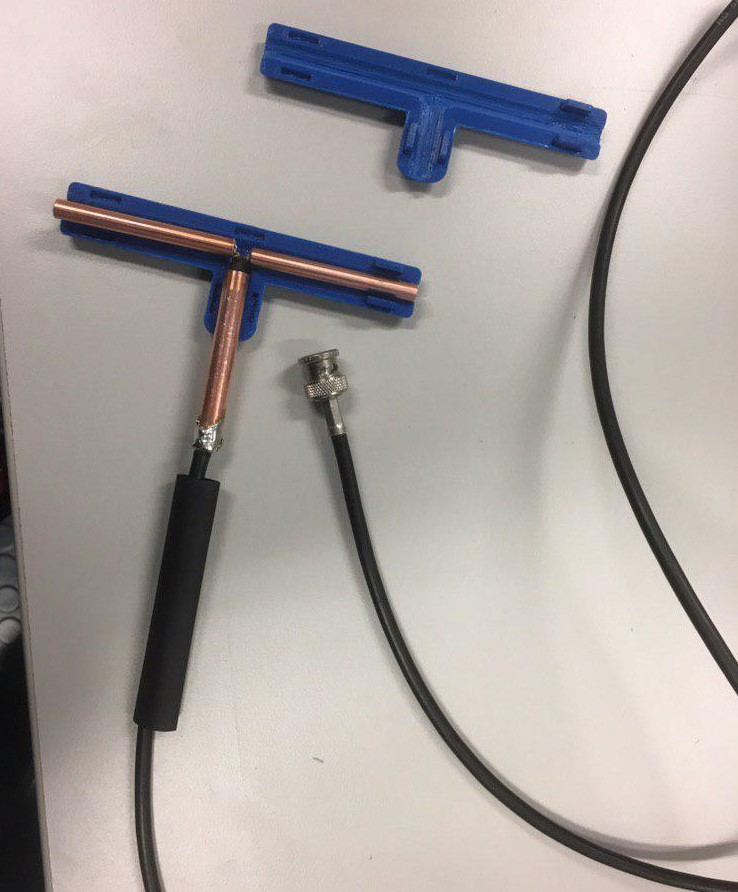
\includegraphics[scale=0.25]{Ant_innen_1}
	\centering
	\caption{Aufbau der ersten gebauten Antenne mit Antennengehäuse und Innenleben.}
\end{figure}
Mit den ersten zwei fertigen Antennen wurden erste Probemessungen gemacht um zu sehen ob in dem erwarteten Frequenzbereich ein Intensität Extremum zu sehen war. Jedoch konnte man im Frequenzband nichts auffallendes erkennen. Was jedoch beobachtet werden konnte war ein unregelmäßig auftauchender Peak bei einer Frequenz von $2.4$\,GHz. 

\subsection{Tag 2}
Am nächsten Tag wurden weiter versucht das HackRF zum laufen zu bringen und die Antennen ausprobiert. Mögliche Lösungen für das Problem der Antennen war eine Entfernung des Gehäuses welche aber zu keinen besseren Ergebnissen geführt hat. Auch andere Positionen im Raum führten zum selben Ergebnis, dass sich keine besondere Frequenz ergab. Es machte sich jedoch schnell bemerkbar, dass der Raum einem Resonator entspricht und kleine Änderungen im Aufbau des Raum größere Unterschiede bezüglich der Übertragenen Leistung machte. Da kein Messgerät zur Messung der Antennengüte vorhanden war wurde versucht die Frequenz durch \textcolor{red}{Erik wie habt ihr das gemacht?}.
\subsection{Tag 3}
Am Mittwoch war das HackRF einsetzbar da wir dieses nun über einen anderen Computer als das Rasberry Pie betrieben. Dies nutzten wir um eine erste Polarisationsmessungen durchzuführen. Auch hier zeigte sich, dass Bewegung von Personen im Raum oder das öffnen eines Fensters die Messwerte stark beeinflusste. Im laufe des Tages erhielten wir ein \textcolor{red}{Name des Geräts?} mit dem die Güte der Antenne gemessen werden konnte. Hier stellte sich heraus die Antennen insgesamt sehr unzuverlässig waren und keine wirklich guten Frequenzen besaßen. Da zusätzlich ein Kurzschluss bei einer der Antennen auftrat wurden zwei neue mit einem Optimierten Design erstellt. Dieses neue Design hatte kein Kupferrohr senkrecht zum Dipol sondern wurde direkt mit einem \textcolor{red}{Steckername} versehen. Beim Test der neuen Antennen zeigt sich eine deutliche Verbesserung zur ersten Generation. Mit Hilfe des \textcolor{red}{Name des Geräts?} konnte ein recht genau gezeugt werden, dass unsere Antennen im erwarteten Bereich besonders gut senden können. Da beide trotzdem leichte Unterschiede in der Frequenz auftraten wurde eine mithilfe eines eingebauten Kondensators auf die andere genormt. 
\subsection{Tag 4}
Mit den nun aufeinander genormten Antennen wurde beschlossen sich auf eine  Polarisationsmessung und eine Abstandmessung zu beschränken und die Messung der Strahlungscharakteristik wegzulassen. Da jedoch auffällig war wie Problematisch die Umgebung des Labors war wurden diese Messungen drinnen so wie draußen im Garten der Physik und am Parkplatz vor dem Westbau durchgeführt.
\subsection{Tag 5}
Am letzten Tag wurden noch zusätzliche Messungen zum Abstand und zur Polarisation im Großen Hörsaal durchgeführt. Da die Messungen im Labor bis dahin wegen Bewegung von Personen sehr ungenau war wurde hier nochmal eine Messung durchgeführt um zu zeigen wie groß die Schwankungen sind und eine bei der sich wirklich nichts verändert.
\begin{figure}[h]
	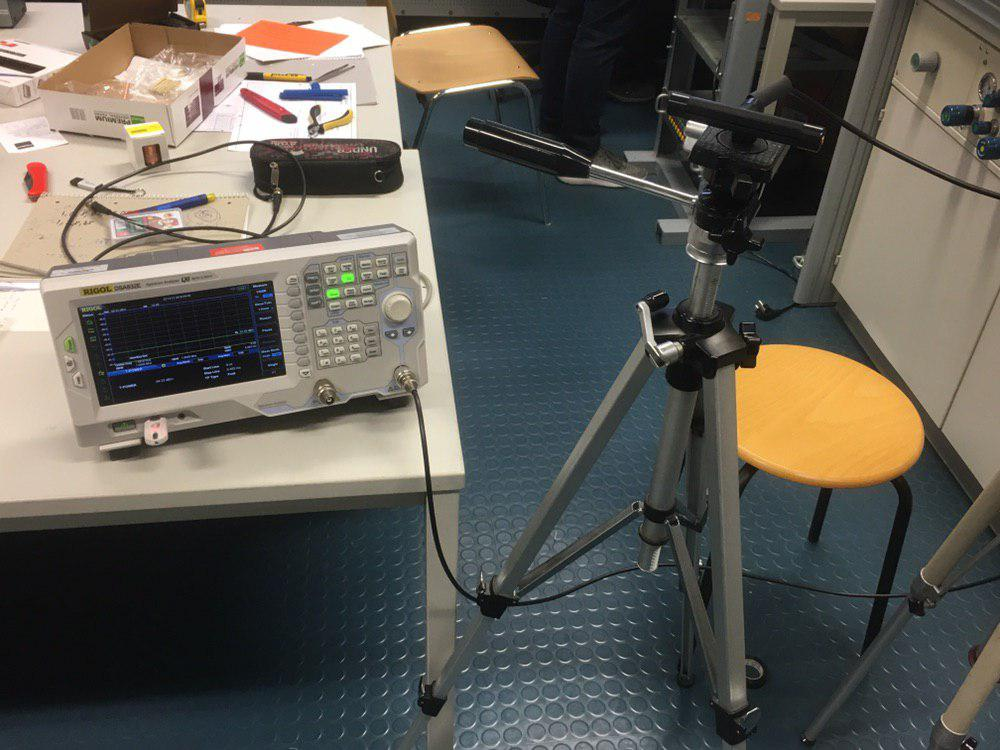
\includegraphics[scale=0.3]{Ant_Fktgen}
	\centering
	\caption{Gebaute Antenne auf dem Stativ und an den Frequenzgenerator angeschlossen.}
\end{figure}
\begin{figure}[h]
	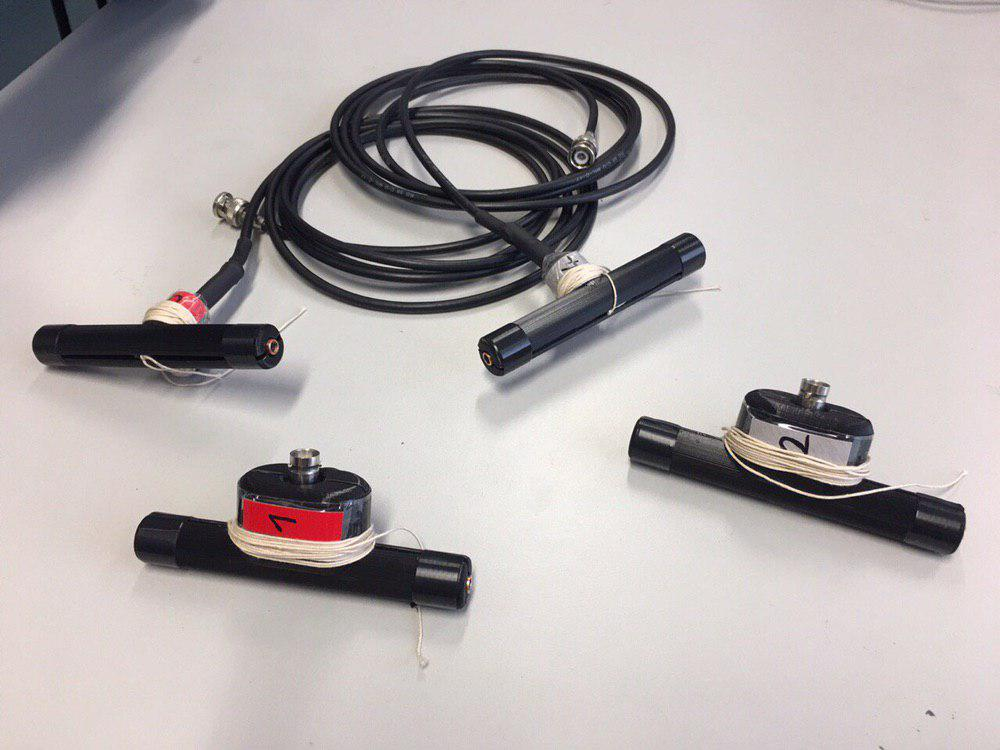
\includegraphics[scale=0.3]{Ant_12}
	\centering
	\caption{Beide Antennen Generationen nebeneinander. Hinten die erste Generation vorne die 2.Generation}
\end{figure}
\begin{figure}[h]
	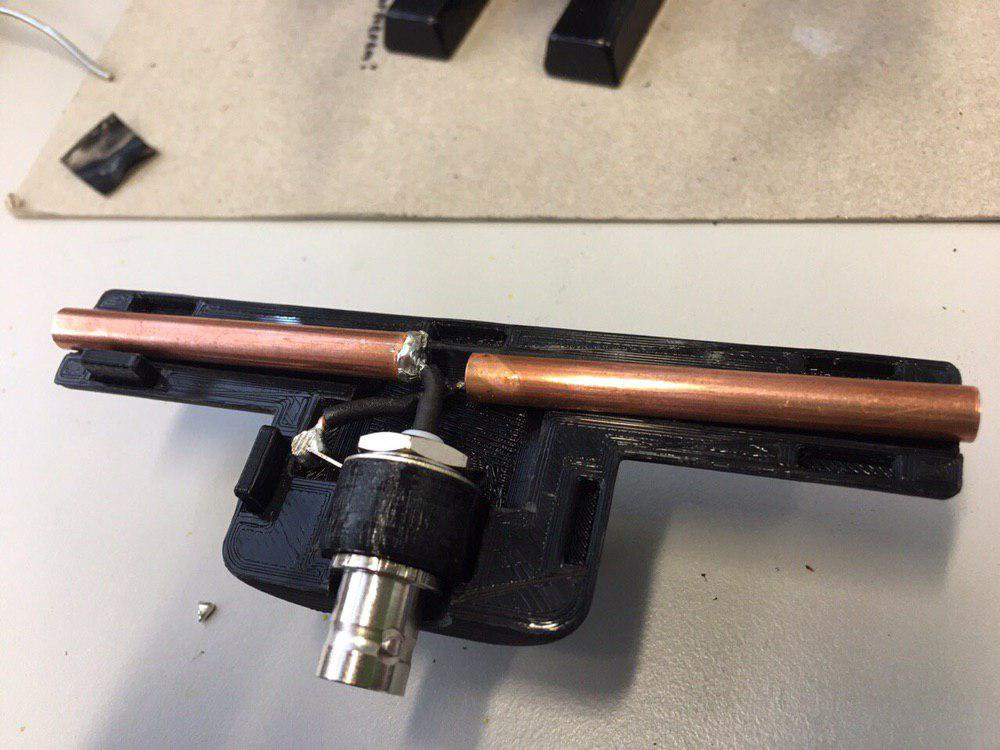
\includegraphics[scale=0.3]{Ant_innen_2}
	\centering
	\caption{Innerer Aufbau der 2.Antennengeneration. Im Bild die genormte Antenne mit kleinem Kondensator an der Seite.}
\end{figure}

\section{Versuchsaufbau für die Messungen}

\subsection{Die Antennen}

Für die Ausgewerteten Messungen haben wir nun ausschließlich die neuen Antennen verwendet. Diese haben im Gegensatz zu dem alten Modell keinen Balun (bestehend aus einer Kupferröhre um das Signalkabel) mehr.\par
Die Antennen bestehen also nur aus zwei Kupferrohren, die jeweils an die Leitung beziehungsweise den Schirm eines Gehäuseanschlusses für BNC Stecker gelötet wurden. Diese Konstruktion wird in einem 3D-gedruckten Gehäuse montiert, sodass die Röhrchen parallel zueinander und orthogonal zum Signalkabel sind. Der nun im Gehäuse eingebaute BNC-Kabel-Anschluss kann nun wie bei anderen kompatiblen Geräten (Oszilloskop, Spectrum Analyzer, etc.) angeschlossen werden. Dieses Design ist also nicht mehr an ein Kabel gebunden, was den Vorteil hat, dass die Länge variabel ist und ein schlechtes Kabel schnell und leicht ausgetauscht werden kann.\par
Die Plastikgehäuse wurden absichtlich so designet, dass sie ohne Metallteile zusammengebaut werden könnte, da diese die Strahlungscharakteristik beeinträchtigen könnten. Der Kunststoff selbst ist sehr dünn und schien keinen Einfluss auf die Messungen nehmen, dies haben wir rein qualitativ überprüft, indem wir das empfange Signal ohne Gehäuse mit dem mit Gehäuse verglichen haben und keinen unterschied feststellen konnten.\par
Außerdem haben die Gehäuse eine Befestigung mit Stativ-Gewinde, sodass sie an Standartmäßigen Fotokamera-Stativen befestigt werden können.

\subsection{Der Aufbau zur Vermessung}

Für die jeweiligen Messung haben wir die beiden Antennen an Stativen befestigt und gegenüber voneinander platziert. Die Gehäuse der Antennen wurden an einer dafür vorgesehenen Öse mit einer Schnur verbunden, um die Parallelität der Antennen bei der Anstandsmessung beziehungsweise einen akkuraten Winkel bei der Polarisationsmessung zu gewährleisten.\par
Beide Antennen wurden an den Spectrum Analyzer angeschlossen. Der Spectrum Analyzers schickt nun ein Signal mit nacheinander verschiedenen Frequenzen durch das gesamte Frequenzband des Spectrum Analyzers an die Sender-Antenne und zeichnet die Intensität des von der Empfänger-Antenne kommenden Signals auf.\par
Ein Vorteil an dieser Messung gegenüber dem Senden einer Frequenz über das Hack-RF ist, das wir auch sofort Störsignale, die von der Antenne empfangen werden feststellen können und damit ausschließen können, dass wie so ein Störsignal mit in die Messung einbeziehen. Hierbei sind Störsignale wie z.B. WLAN oder andere zeitlich nicht konstante Funksignale gemeint. Außerdem 

\subsection{Polarisation}
Zur Messung der Polarisation wurden die Beiden Antennen in einem festen Abstand voneinander auf dem jeweiligen Stativ befestigt. Zum Test ob die Antennen Rechtwinkelig voneinander sind wurde ein Faden genutzt der zwischen beiden Antennen gespannt wurde und dann mit Hilfe eines Geodreiecks ein Rechter Winkel zwischen Antenne und Faden gemessen wurde. Der Sender und Empfänger wurden dann an das Frequenzspektrometer angeschlossen. Zur eigentlichen Messung wurde die Leistungsdifferenz zwischen Sender und Empfänger bei unterschiedlichen Winkeln des Empfängers gemessen.


\bibliographystyle{plain}
\bibliography{literature}
\addcontentsline{toc}{section}{Literatur}

\end{document}
